\section{Look Ahead}
\subsection{Theory of Operation}

The look ahead node is responsible for obstacle detection. The node
subscribes to lidar data and uses trigonometric functions to check for
obstacles within a bounded box.  The box's dimensions are currently 1m
in front of the robot and .25m on either side. 

The node constantly publishes to the obstacles topic using a custom
message type of ``Obstacle''.  The Obstacle message and the
subscribers of the obstacle topic are described in Custom Message
Specifications section.

In order to perform its job the Look Ahead node subscribes to the
lidar data published with message type sensor\_msgs/laserscan. This message
includes information about each laser ping's distance and intensity as
well as information about the laser range finder device itself.  In
our case, the lidar is set to do 181 pings on every sweep with spacing
of 1 degree per ping.  This works out to a sweep from -90$^\circ$ to
90$^\circ$ in the robots base coordinate frame.

When an obstacle is detected in the box the obstacles boolean in the
Obstacle message type is set to true. The algorithm also calculates
the closest of the obstacle pings and puts that number in the distance field
of the Obstacle message type. When no obstacles are detected obstacles
is set to false and distance is set to 0.0.

\subsubsection{Implementation Decisions}

To account for the possibility of more pings per sweep or sweeps of
smaller degrees we have constants that are defined globally at the top
of the file.  This gives us a single place to change fundamental
parameters of the program.  We could potentially move these into a
configuration file to prevent the need to recompile when new settings
are desired.

\subsubsection{Bounding Box Algorithm}
To determine if a ping is within the box dimensions the trigonometric
functions are used to determine the bounds of the box.  For each ping
a maximum distance is computed.  If the ping distance is larger than this
value then it is ignored. If the ping distance is less it is
considered an obstacle.  The minimum of all pings within the distance
thresholds is returned as the distance.

\FloatBarrier
\begin{figure}[h]
  \centering
  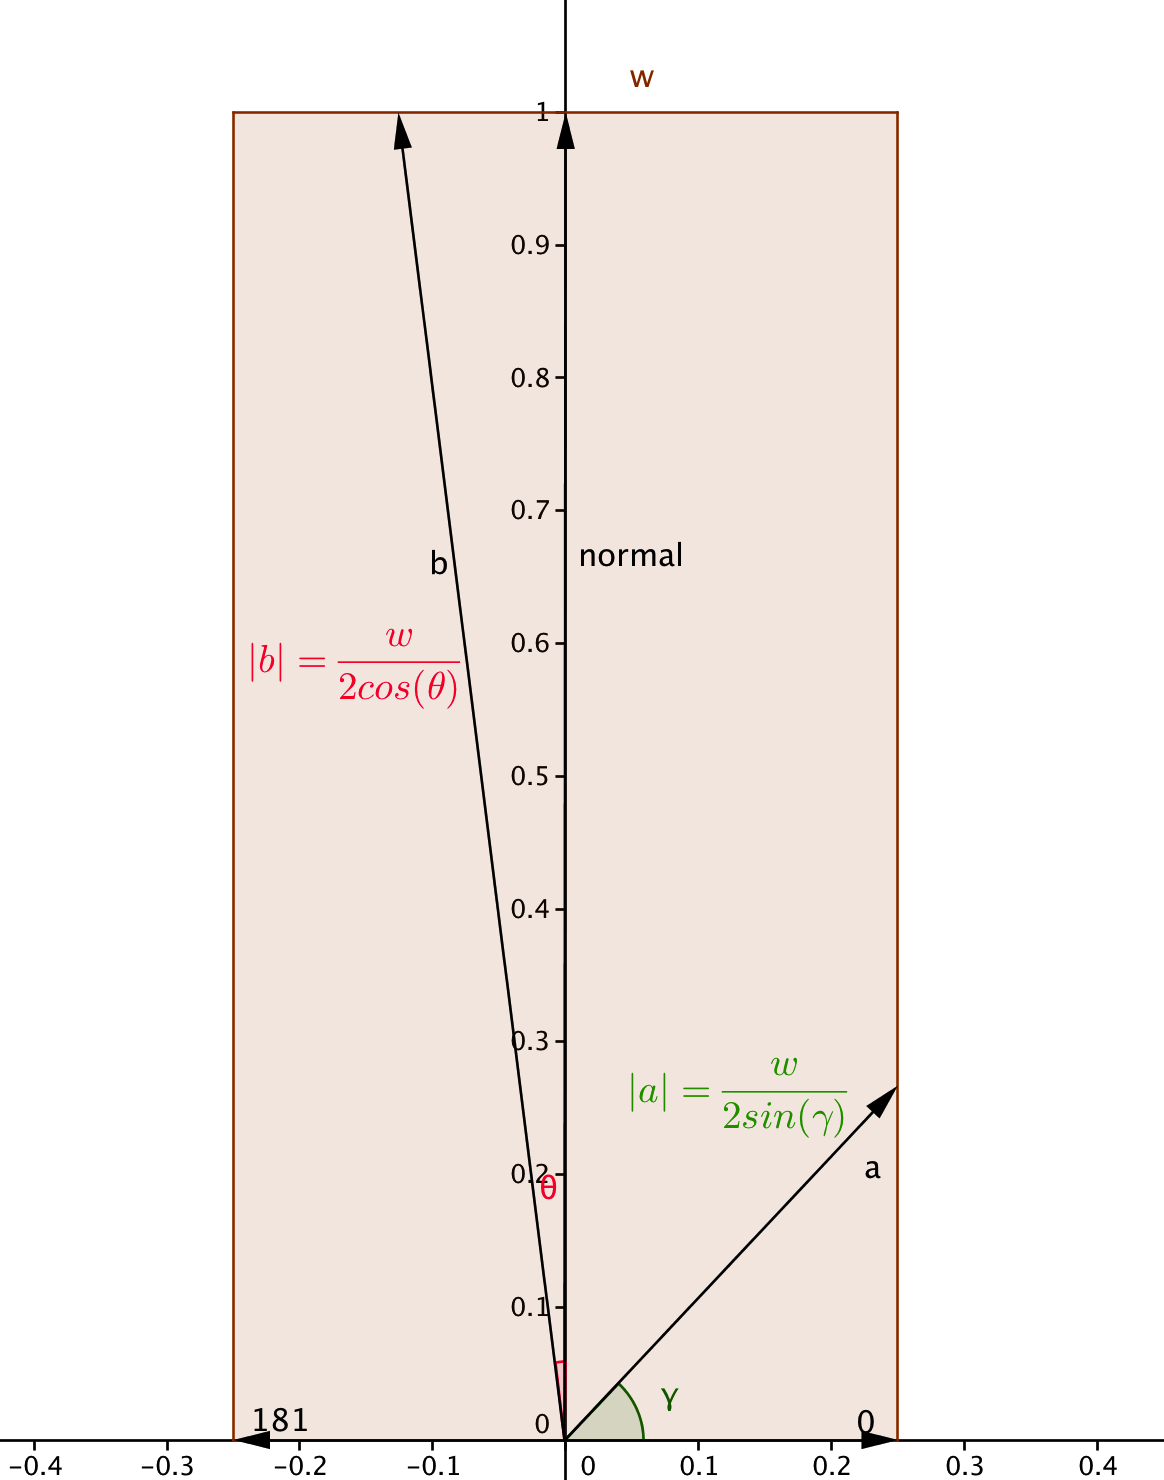
\includegraphics[height=4.5in]{Look_Ahead_Bounding_Box.png}
  \caption{Calculations for laser ping distances}
  \label{fig:lookAheadLaserPingDistances}
\end{figure}
\FloatBarrier

In this figure a laser ping from each of the two region types is shown
along with the function used to calculate the maximum distance.

\FloatBarrier
\begin{figure}[h]
  \centering
  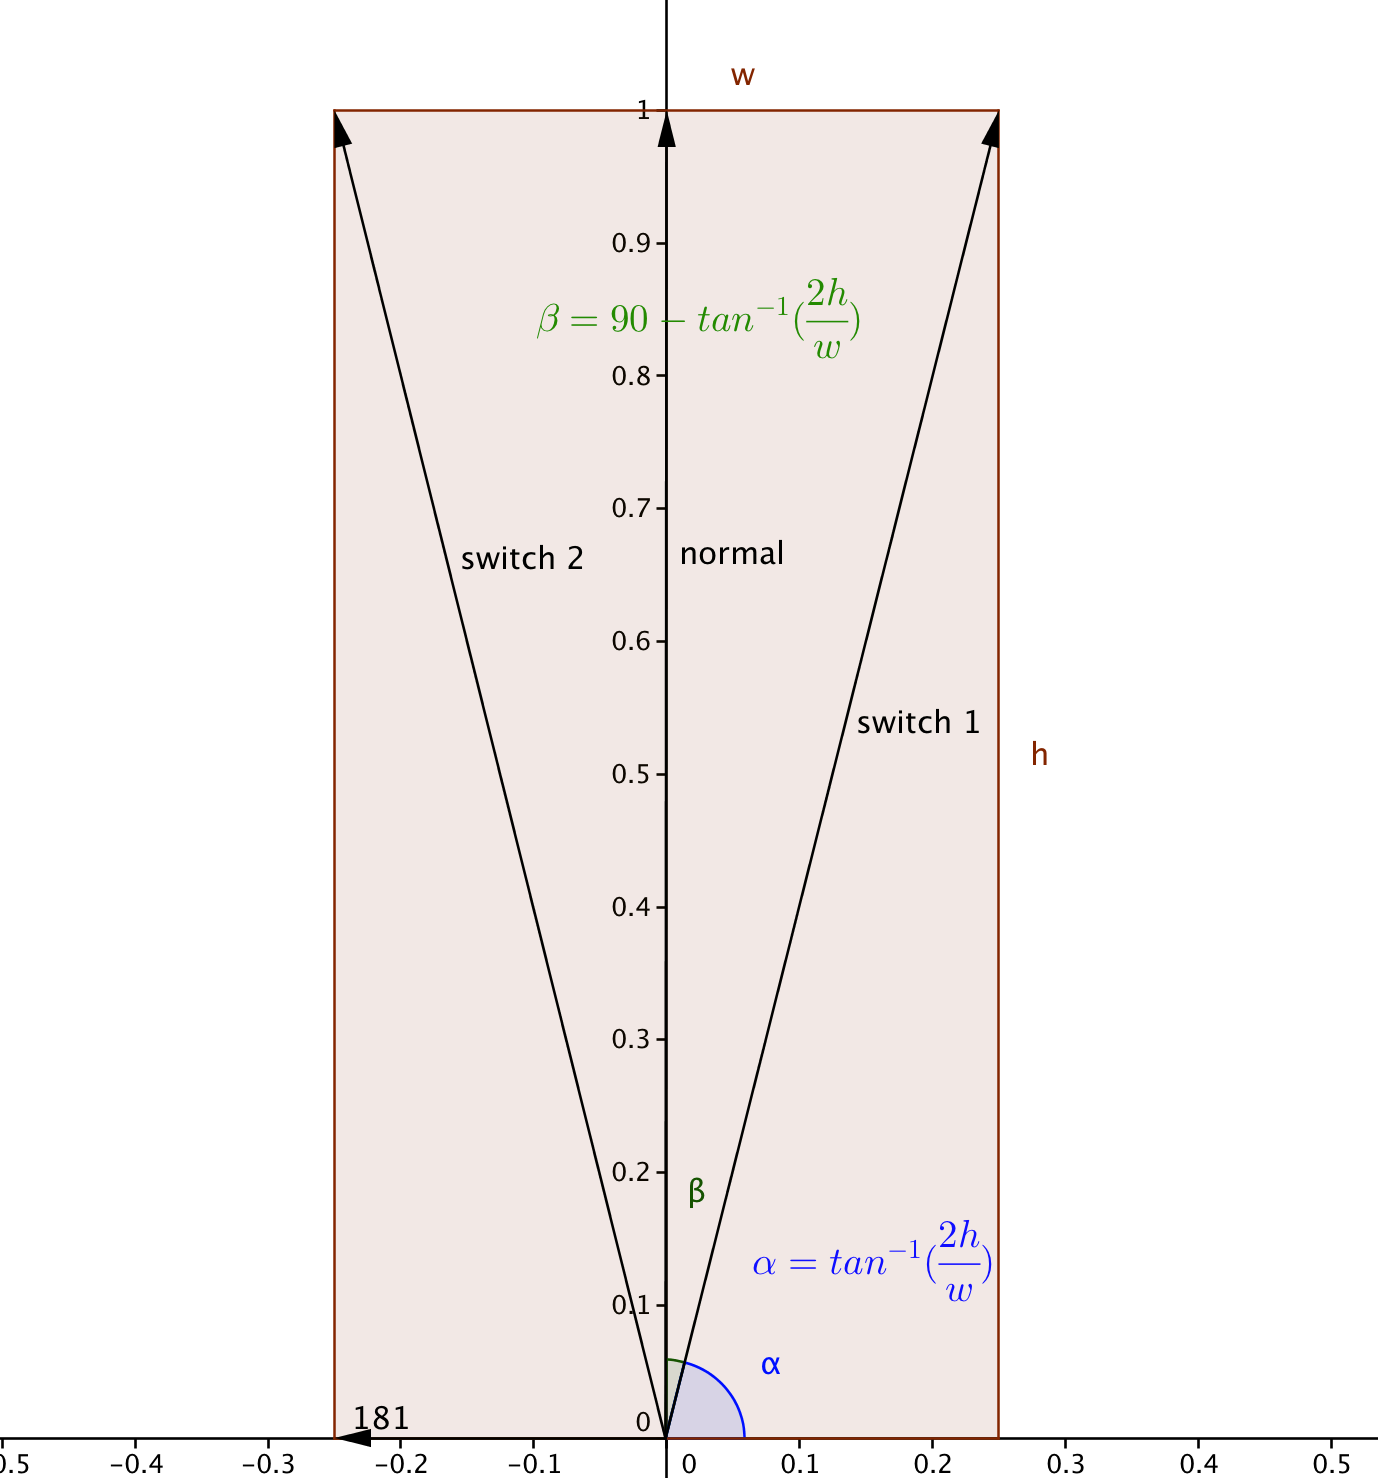
\includegraphics[height=4.5in]{look_ahead_bounding_box_transitions.png}
  \caption{Calculations for the transition angles}
\end{figure}
\FloatBarrier

This figure shows what how the transition angles are calculated.
After the ping corresponding to one of the transition angles is surpassed,
the calculations for the next set of pings switches between the two
equations shown in figure 3.

\subsection{Observations}

\subsubsection{Lidar Problems}

Sometimes the LIDAR data would drop out. To fix this problem we would restart the computer and it would usually comeback once the computer had started back up. We are not sure what is causing the problem, however, one of our theories is that multiple people trying to run their code causes the problem. If one person starts the cwru\_bringup\_no\_tele launch file then the two will conflict and the console will print LIDAR timeout messages. After this occurs its possible that internal state variables become corrupted and so the LIDAR code on the robot fails to act properly until a restart.

Another theory is that bugs in the various groups' code such as memory leaks and segfaults leave subprocesses running in the background. These zombie processes may be causing interference. Between the wo the first theory seems more likely. Especially since the bringup launch script can be run in a background process or through a screen session.

\subsection{Unimplemented Functions}

Before spring break we had plans to update look ahead so that it could detect obstacles before going into a spin segment and so that it could detect obstacles more accurately on an arc. We had planned on taking in the path segment list and detecting when the next segment would be a spin. If we detected any obstacles in the area the robot would move through while executing the spin we would stop on the segment before the spin and wait until the obstacle moved or we replanned. This would have avoided the part of the problem with the LIDAR's blind spots.

In addition for the last demo we found that because of the very small path segment distances our bounding box algorithm, would often give responses too late to do anything but a hard stop. Our current approach is to stop the robot only if the distance to the closest obstacle is within our path segment distance. This needs to be changed to within some distance along the entire path. With the short segments published by our path planner the robot won't stop until its so close its essentially already collided with it. However, if the costmap were working this may become a moot point as that should allow us to detect all obstacles including ones from the kinect and dynamically steer around them.






